\documentclass[aspectratio=169]{beamer}
\usepackage{pgfgantt}
\usepackage{xcolor}
\usepackage{tikz}
\usetikzlibrary{shapes,arrows,positioning,fit,backgrounds,calc,decorations.pathreplacing,patterns,shadows,3d,matrix}
\usepackage{amsmath}
\usepackage{amssymb}
\usepackage{xcolor}
\usepackage{pgfplots}
\pgfplotsset{compat=1.17}

\usepackage{booktabs}
\usepackage{array}
\usepackage{colortbl}

% Beamer theme
\usetheme{Madrid}
\usecolortheme{default}

% UQAC institutional green — overrides Madrid's default blue
\definecolor{uqacgreen}{RGB}{0,99,65}
\setbeamercolor{structure}{fg=uqacgreen}
\setbeamercolor{palette primary}{bg=uqacgreen,fg=white}
\setbeamercolor{palette secondary}{bg=uqacgreen!80!black,fg=white}
\setbeamercolor{palette tertiary}{bg=uqacgreen!60!black,fg=white}
\setbeamercolor{palette quaternary}{bg=uqacgreen!40!black,fg=white}
\setbeamercolor{frametitle}{bg=uqacgreen,fg=white}
\setbeamercolor{title}{bg=uqacgreen,fg=white}
\setbeamercolor{block title}{bg=uqacgreen,fg=white}
%\setbeamercolor{block title alerted}{bg=uqacgreen!70!black,fg=white}
\setbeamercolor{section in head/foot}{bg=uqacgreen!80!black,fg=white}
\setbeamercolor{subsection in head/foot}{bg=uqacgreen!60!black,fg=white}

% Custom colors matching previous diagrams
\definecolor{primary}{RGB}{0,99,65}
\definecolor{secondary}{RGB}{255,102,0}
\definecolor{accent1}{RGB}{0,153,76}
\definecolor{accent2}{RGB}{204,0,102}
\definecolor{accent3}{RGB}{153,0,204}
\definecolor{lightgray}{RGB}{240,240,240}
\definecolor{medgray}{RGB}{180,180,180}
\definecolor{darkgray}{RGB}{80,80,80}

\definecolor{risklow}{RGB}{144,238,144}
\definecolor{riskmed}{RGB}{255,255,150}
\definecolor{riskhigh}{RGB}{255,200,100}
\definecolor{riskcrit}{RGB}{255,120,120}

% Define custom styles
\tikzstyle{process} = [rectangle, rounded corners, minimum width=3cm, minimum height=1cm,
    text centered, draw=primary, fill=primary!10, font=\sffamily\small, drop shadow]
\tikzstyle{decision} = [diamond, aspect=2, minimum width=3cm, minimum height=1cm,
    text centered, draw=secondary, fill=secondary!10, font=\sffamily\small, drop shadow]
\tikzstyle{data} = [trapezium, trapezium left angle=70, trapezium right angle=110,
    minimum width=3cm, minimum height=1cm, text centered, draw=accent1, fill=accent1!10,
    font=\sffamily\small, drop shadow]
\tikzstyle{storage} = [cylinder, shape border rotate=90, aspect=0.25, minimum width=2.5cm,
    minimum height=1.5cm, text centered, draw=accent2, fill=accent2!10, font=\sffamily\small, drop shadow]
\tikzstyle{cloud} = [ellipse, minimum width=3cm, minimum height=1.5cm, text centered,
    draw=accent3, fill=accent3!10, font=\sffamily\small, drop shadow]
\tikzstyle{module} = [rectangle, rounded corners, minimum width=4cm, minimum height=2cm,
    text centered, draw=primary, fill=primary!5, line width=1.5pt, font=\sffamily, drop shadow]
\tikzstyle{arrow} = [thick,->,>=stealth,line width=1.5pt]
\tikzstyle{bidiarrow} = [thick,<->,>=stealth,line width=1.5pt]
\tikzstyle{dottedarrow} = [thick,->,>=stealth,dashed,line width=1.5pt]


\titlegraphic{%
    \begin{tikzpicture}[remember picture,overlay]
        \node[anchor=north, xshift=0cm, yshift=0cm] 
            at (current page.north) 
            {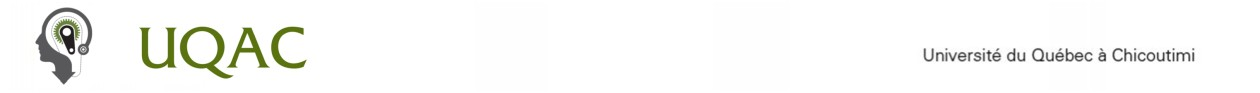
\includegraphics[height=1.2cm]{en-tete1260.jpg}};
    \end{tikzpicture}
    
    \begin{tikzpicture}[remember picture,overlay]
        \node[anchor=south east, xshift=0.3cm, yshift=0.3cm] 
            at (current page.south east) 
            {
\includegraphics[height=2.5cm]{LogoLARI_FINAL.png}};
    \end{tikzpicture}
}
% Add logo to the right side of the frametitle
\addtobeamertemplate{frametitle}{}{%
    \begin{tikzpicture}[remember picture,overlay]
        \node[anchor=north east, xshift=-0.3cm, yshift=0.3cm] 
            at (current page.north east) 
            {
\includegraphics[height=1.2cm]{LogoLARI_FINAL.png}};
    \end{tikzpicture}
}

% Title page information
\title{Titre principal du sujet \& continue sur la ligne suivante}
\subtitle{Sous-titre du projet de recherche}
\author{Auteur 1, Auteur 2, Auteur 3, ...}
\institute{Université du Québec à Chicoutimi \& Partenaire industriel}
\date{\today}

\begin{document}

% Title slide
\begin{frame}
\titlepage
\end{frame}

% Table of contents
\begin{frame}{Outline}
\tableofcontents
\end{frame}

% ==================================================================================
% SECTION 1: INTRODUCTION
% ==================================================================================
\section{Introduction}

\begin{frame}{Introduction}
\begin{block}{Le défi principal}
Défi majeur
\end{block}

\begin{columns}[t]
\column{0.48\textwidth}
\textbf{Contexte réel actuel:}
\begin{itemize}
    \item \textcolor{accent2}{\textbf{XYZ}} energy consumption
    \item \textcolor{accent2}{\textbf{$\sim$1\%}} of global CO$_2$ emissions
    \item Process largely unchanged for last years
    \item Reactive, operator-dependent control
\end{itemize}

\column{0.48\textwidth}
\textbf{Industry Pressures:}
\begin{itemize}
    \item Carbon emission regulations
    \item Energy cost volatility
    \item Production efficiency demands
    \item Sustainability requirements
\end{itemize}
\end{columns}

\vspace{0.3cm}
\begin{alertblock}{Critical Need}
\textbf{Transformative approach} beyond incremental improvements → Intelligent, predictive, autonomous control
\end{alertblock}

\vspace{0.2cm}
\begin{center}
\textit{From reactive adjustments to proactive optimization}
\end{center}
\end{frame}

% ==================================================================================
% SECTION 2: PROBLEMATIC AND NEEDS
% ==================================================================================
\section{Problématique \& besoins}

\begin{frame}{Problématique \& besoins industriels}
\begin{columns}[t]
\column{0.48\textwidth}
\textbf{Current Limitations:}
\begin{itemize}
    \item \textcolor{accent2}{Manual control}: operator experience
    \item \textcolor{accent2}{Limited visibility} into unmeasurable states
    \item \textcolor{accent2}{Reactive strategies} → late interventions
    \item Complex multi-physics interactions not fully exploited
\end{itemize}

\column{0.48\textwidth}
\textbf{Industry Needs:}
\begin{itemize}
    \item \textcolor{accent1}{Predictive capability} (hours to days ahead)
    \item \textcolor{accent1}{Real-time optimization} balancing multiple objectives
    \item \textcolor{accent1}{Energy cost reduction} while maintaining quality
    \item \textcolor{accent1}{Carbon footprint reduction}
    \item \textcolor{accent1}{Extended cell life}
\end{itemize}
\end{columns}
\end{frame}

\begin{frame}{Solutions}

\begin{columns}[t]
\column{0.45\textwidth}
\vspace{-0.7cm}
\begin{block}{The Gap}
\textbf{Traditional approaches} (empirical rules, simple control) \textbf{vs.} Modern capabilities (AI, digital twins, predictive optimization)
\end{block}

%\vspace{0.1cm}
\begin{alertblock}{Solution Direction}
Integrate \textbf{physics knowledge} + \textbf{data-driven AI} + \textbf{world-model policies} → Autonomous, self-optimizing system
\end{alertblock}

\begin{alertblock}{Vision}
Smart, Predictive, Efficient \& Carbon-Free Aluminium Production
\end{alertblock}


\column{0.5\textwidth}
    \begin{figure}[h]
        \centering
        
\includegraphics[width=\linewidth]{LogoLARI_FINAL.png}
        \caption{System integration}
        \label{fig:scenarios_result}
    \end{figure}
\end{columns}


\end{frame}

% ==================================================================================
% SECTION 3: OBJECTIVES
% ==================================================================================
\section{Objectifs principaux}

\begin{frame}{Objectifs des travaux de recherche}


\begin{columns}[t]
\column{0.48\textwidth}
\textbf{X Objectifs intégrés:}

\vspace{0.2cm}
\begin{enumerate}
    \item \textcolor{primary}{\textbf{Smart Operation}}
    \begin{itemize}
        \scriptsize
        \item Autonomous AI-driven control
        \item Multi-agent coordination
        \item Self-learning from plant data
    \end{itemize}
    
    \vspace{0.1cm}
    \item \textcolor{accent1}{\textbf{Predictive Capability}}
    \begin{itemize}
        \scriptsize
        \item Multi-horizon forecasting (15min - 7 days)
        \item Early disruption detection
        \item Proactive intervention
    \end{itemize}
\end{enumerate}

\column{0.48\textwidth}
\vspace{0.85cm}
\begin{enumerate}
    \setcounter{enumi}{2}
    \item \textcolor{secondary}{\textbf{Energy Efficiency}}
    \begin{itemize}
        \scriptsize
        \item \textbf{Target: 5-10\% reduction}
        \item Optimized thermal/current management
        \item Economic MPC
    \end{itemize}
    
    \vspace{0.1cm}
    \item \textcolor{accent2}{\textbf{Carbon Elimination}}
    \begin{itemize}
        \scriptsize
        \item \textbf{Target: 20-30\% PFC reduction}
        \item Predictive effect prevention
        \item Renewable energy alignment
    \end{itemize}
\end{enumerate}
\end{columns}

\vspace{0.3cm}
\begin{alertblock}{Convergence}
Next-generation production: \textbf{self-optimizing, environmentally sustainable, economically superior}
\end{alertblock}
\end{frame}

\begin{frame}{Research Methods \& Approach}
\vspace{-0.7cm}
    \begin{figure}[h]
        \centering
        
\includegraphics[trim={0cm 0cm 0cm 1.8cm}, clip, width=0.8\linewidth]{LogoLARI_FINAL.png}
        \caption{System integration}
        \label{fig:architecture_scenarios_result}
    \end{figure}
\end{frame}

% ==================================================================================
% SECTION 4: METHODS
% ==================================================================================
\begin{frame}{Research Methods \& Approach}

\vspace{0.2cm}

\begin{block}{Phase 1: Mitigation / Temporal behavioral prediction / Open loop}
\centering
\scriptsize
\textbf{Data/Needs (Ph.D.1/2)} $\rightarrow$ \textbf{Time series model (Ph.D.1) \& Cyclic model (Ph.D.2)} $\rightarrow$ \textbf{Prediction} $\rightarrow$ \textbf{Field Deployment}
\end{block}


\begin{block}{Phase 2: Integration Strategy}
\centering
\scriptsize
\textbf{Data (M1)} $\rightarrow$ \textbf{Digital Twin (Ph.D. 1) \& Policies (Ph.D. 2)} $\rightarrow$ \textbf{Optimization (M2, M3)} $\rightarrow$ \textbf{Field Deployment}
\end{block}



\end{frame}

\section{Methods}

\begin{frame}{Research Methods \& Approach}
\vspace{-0.6cm}
\begin{columns}[t]
\column{0.48\textwidth}
\textbf{1. Hybrid Digital Twin (Ph.D. 1)}
\begin{itemize}
    \scriptsize
    \item \textcolor{primary}{Physics-based models}: somethings
    \item \textcolor{accent1}{AI acceleration}: somethings
    \item Real-time capability ($<$ 1 min)
\end{itemize}

\vspace{0.2cm}
\textbf{2. World-Model Policies (Ph.D. 2)}
\begin{itemize}
    \scriptsize
    \item \textcolor{primary}{Forecasting}: LSTM-Transformer
    \item \textcolor{accent1}{Anomaly detection}: GAN-based
\end{itemize}

\column{0.48\textwidth}
%\vspace{-0.5cm}
\textbf{3. Data Foundation (M1)}
\begin{itemize}
    \scriptsize
    \item 3+ years historical data
    \item LLM-assisted annotation
    \item 100\% labeled dataset
    \item Feature engineering
\end{itemize}

\textbf{4. Economic MPC (M2)}
\begin{itemize}
    \scriptsize
    \item Multi-objective cost function
    \item Time-varying Faraday efficiency / SEC
    \item Emission costs integration
    \item KPI dashboard (real-time)
\end{itemize}

\vspace{0.2cm}
\textbf{5. Multi-Objective Optimization (M3)}
\begin{itemize}
    \scriptsize
    \item MOBFO, MOALO, K-RVEA algorithms
    \item Knowledge-guided optimization
    \item Pareto front analysis
    \item Decision support system
\end{itemize}


\end{columns}
\end{frame}



% ==================================================================================
% SECTION 5: OVERALL PROJECT GANTT (moved here as timeline visualization)
% ==================================================================================
\section{Timeline}

\begin{frame}[fragile]{Project Timeline}
\begin{center}
\vspace{-0.4cm}
\scalebox{0.58}{
\begin{ganttchart}[
    x unit=0.38cm,
    y unit title=0.6cm,
    y unit chart=0.5cm,
    vgrid,
    hgrid,
    title height=1,
    bar height=0.6,
    group height=0.6,
    bar/.append style={fill=primary!80},
    group/.append style={fill=secondary!80},
    milestone/.append style={fill=accent2, rounded corners=3pt},
    title label font=\tiny,
    bar label font=\scriptsize,
    group label font=\scriptsize\bfseries,
    milestone label font=\tiny,
]{1}{60}

% Title - Years
\gantttitle{Project Timeline (60 Months)}{60} \\
\gantttitle{Year 1}{12}
\gantttitle{Year 2}{12}
\gantttitle{Year 3}{12}
\gantttitle{Year 4}{12}
\gantttitle{Year 5}{12} \\

% Ph.D. Students
\ganttgroup{Ph.D. 1: Digital Twin}{1}{36} \\
\ganttbar{Physics Models}{1}{12} \\
\ganttbar{AI Acceleration}{13}{24} \\
\ganttbar{Validation \& Thesis}{25}{36} \\

\ganttgroup{Ph.D. 2: Policies}{1}{36} \\
\ganttbar{Forecasting}{1}{12} \\
\ganttbar{Agent-Based Models}{13}{24} \\
\ganttbar{Field Deploy \& Thesis}{25}{36} \\

% Master's Students
\ganttgroup{M1: Data}{1}{24} \\
\ganttbar{Pipeline \& Annotation}{1}{18} \\
\ganttbar{Finalization \& Thesis}{19}{24} \\

\ganttgroup{M2: EMPC}{21}{44} \\
\ganttbar{Formulation \& Impl.}{21}{32} \\
\ganttbar{Validation \& Thesis}{33}{44} \\

\ganttgroup{M3: Multi-Obj Opt}{41}{60} \\
\ganttbar{Algorithms}{41}{52} \\
\ganttbar{Analysis \& Thesis}{53}{60} \\

% Milestones
\ganttmilestone{Data Ready}{24} \\
\ganttmilestone{Twin Ready}{36} \\
\ganttmilestone{2 Ph.D. Defenses}{36} \\
\ganttmilestone{M2 Defense}{44} \\
\ganttmilestone{Project Complete}{60}

% Links
\ganttlink{elem0}{elem1}
\ganttlink{elem1}{elem2}
\ganttlink{elem3}{elem4}
\ganttlink{elem4}{elem5}

\end{ganttchart}
}

\end{center}

%\vspace{-0.3cm}
%\begin{block}{\tiny Key Features}
%\scriptsize
%\textbf{Sequential Ph.D.s:} Knowledge transfer (Ph.D. 1 → Ph.D. 2) | 
%\textbf{Staggered Masters:} M1→M2→M3 | 
%\textbf{Peak:} 4 students in Year 3
%\end{block}

\end{frame}

% ==================================================================================
% SECTION 6: RESOURCES
% ==================================================================================
\section{Resources}

\begin{frame}{Resource Allocation}
\begin{columns}[t]
\column{0.48\textwidth}
\textbf{Human Resources:}

\vspace{0.2cm}
\begin{table}
\scriptsize
\begin{tabular}{|l|c|c|}
\hline
\textbf{Student} & \textbf{Duration} & \textbf{Stipend/yr} \\
\hline
Ph.D. 1 & 36 mo & \$40,000 \\
Ph.D. 2 & 36 mo & \$40,000 \\
M1 & 24 mo & \$35,000 \\
M2 & 24 mo & \$35,000 \\
M3 & 20 mo & \$35,000 \\
\hline
\end{tabular}
\end{table}

\vspace{0.2cm}
\textbf{Support Staff:}
\begin{itemize}
    \scriptsize
    \item Technical staff: 0.5 FTE
    \item PI supervision: 20\% FTE
\end{itemize}

\vspace{0.2cm}
\textbf{Active Students by Year:}
\begin{itemize}
    \scriptsize
    \item Year 1: 3 | \textcolor{accent2}{\textbf{Year 2: 4}} | Year 3: 3
    \item Year 4: 2 | Year 5: 1
\end{itemize}

\column{0.48\textwidth}
\textbf{Computational Resources:}
\begin{itemize}
    \scriptsize
    \item GPU hours: 43,000 (A100 equiv.)
    \item CPU hours: 69,000 (core-hours)
    \item Storage: 20 TB
    \item Cloud budget: \$40,000
\end{itemize}

\vspace{0.2cm}
\textbf{On-Site Industrial Work:}
\begin{itemize}
    \scriptsize
    \item Ph.D. students: 5 days/week
    \item M1: 5 days/week (data access)
    \item M2, M3: 5 days/week
\end{itemize}

\vspace{0.2cm}
\textbf{Meetings:}
\begin{itemize}
    \scriptsize
    \item Weekly: Individual supervision (1h)
    \item Monthly: Full team (3h)
    \item Quarterly: Stakeholder reviews
\end{itemize}
\end{columns}

%\vspace{0.2cm}
%\begin{alertblock}{Strategic Allocation}
%\scriptsize Peak resources in Year 3 coincide with integration phase and knowledge transfer from Ph.D. 1 to Ph.D. 2
%\end{alertblock}
\end{frame}

% ==================================================================================
% SECTION 7: BUDGET
% ==================================================================================
\section{Budget}

\begin{frame}{5-Year Budget Summary}


\vspace{0.2cm}
%\scalebox{1.2}{
\begin{table}
\scriptsize
\begin{tabular}{|l|r|r|r|r|r|r|}
\hline
\rowcolor{primary!20}
\textbf{Category} & \textbf{Amount (CAN)} & \textbf{MITACS} & \textbf{Alouette} & CalculCanada & PROMPT & NSERC \\
\hline
\multicolumn{2}{|l|}{\textit{Personnel}} & & & & &\\
Ph.D. Stipends & \$240,000 & \$7500x16u & \$7500x16u+tx& & &\\
Master's Stipends & \$210,000 & \$7500x14u & \$7500x14u+tx& & &\\ 
%Technical Staff & \$200,000 \\
\hline
\textbf{Personnel Total} & \textbf{\$450,000} & \textbf{\$225,000} & \textbf{\$225,000+tx} & & &\\
\hline
\multicolumn{2}{|l|}{\textit{Equipment \& Computing}} & & &  & &\\
%Workstations/Servers & \$40,000 \\
GPU Cloud Computing & \$40,000 & & &\$40,000  & &\\
%Software Licenses & \$25,000 \\
\hline
\textbf{Equipment Total} & \textbf{\$40,000} & & & \$40,000 & &\\
\hline
%\multicolumn{2}{|l|}{\textit{Travel \& On-Site}} \\
%Conferences & \$64,000 \\
%Industrial Visits & \$50,000 \\
%\hline
%\textbf{Travel Total} & \textbf{\$114,000} \\
\hline
\textcolor{accent2}{\textbf{GRAND TOTAL}} & \textcolor{accent2}{\textbf{\$490,000}} & \textbf{\$225,000} & \textbf{\$225,000+tx} & \textbf{\$40,000}  & &\\
\hline
\end{tabular}
\end{table}


\end{frame}

% ==================================================================================
% SECTION 8: EXPECTED OUTCOMES (renamed to be before Conclusion)
% ==================================================================================
\section{Expected Outcomes}

\begin{frame}{Expected Outcomes \& Impact}

\vspace{-0.4cm}
\textbf{Scientific Contributions:}
\begin{itemize}
    \scriptsize
    \item Novel hybrid digital twin architecture (never developped)
    \item World-model based policy framework (main innovation)
    \item Benchmark datasets
    \item Multi-objective optimization methods
\end{itemize}

\vspace{0.2cm}
\begin{table}
\tiny
\begin{tabular}{|l|r|}
\hline
Ph.D. Theses & 2 \\
Master's Theses & 3 \\
Journal Papers & 6+ \\
Conference Papers & 10+ \\
Data Papers & 1 \\
Software Packages & 3 \\
\hline
\end{tabular}
\end{table}

\vspace{0.2cm}
\textbf{Knowledge Transfer:}
\begin{itemize}
    \scriptsize
    \item Training materials
    \item User manuals
    \item Industry workshop
    %\item Open datasets (if permitted)
\end{itemize}

\vspace{0.2cm}
\begin{alertblock}{Technology Readiness}
Target: TRL 6-7 (system demonstration, pilot deployment) by project end
\end{alertblock}
\end{frame}

% ==================================================================================
% SLIDE 1: Global Summary
% ==================================================================================
\begin{frame}{Global Summary of the Risk}
\vspace{-0.6cm}
\begin{center}
\begin{tabular}{|l|c|c|c|}
\hline
\rowcolor{primary!20}
\textbf{Category} & \textbf{Max Possible} & \textbf{Achieved Score} & \textbf{Percentage} \\
\hline
\textbf{A. Risk (inverse)} & 2.50 & 1.35 & \cellcolor{riskhigh}54.0\% \\
\hline
\textbf{B. Feasibility} & 2.25 & 1.80 & \cellcolor{risklow}80.0\% \\
\hline
\textbf{C. Timeline} & 1.75 & 1.00 & \cellcolor{riskhigh}57.1\% \\
\hline
\textbf{D. Impact \& Innovation} & 2.00 & 1.80 & \cellcolor{risklow}90.0\% \\
\hline
\textbf{E. Project Management} & 1.25 & 0.96 & \cellcolor{riskmed}76.8\% \\
\hline
\rowcolor{primary!30}
\textbf{TOTAL} & \textbf{9.75} & \textbf{6.91} & \textbf{70.9\%} \\
\hline
\end{tabular}
\end{center}

\vspace{0.3cm}

\begin{columns}[T]
\column{0.48\textwidth}
\textbf{Strengths:}
\begin{itemize}
    \scriptsize
    \item Scientific Innovation: 5/5
    \item Industrial Impact: 5/5
    \item Feasibility: 80\%
\end{itemize}

\column{0.48\textwidth}
\textbf{Concerns:}
\begin{itemize}
    \scriptsize
    \item Technical Risk: 2/5
    \item Buffer Time: 2/5
    \item Timeline Realism: 57\%
\end{itemize}
\end{columns}

\vspace{0.2cm}
\begin{alertblock}{Overall Assessment}
\centering
\textbf{Grade B (70.9\%)} -- Good foundation with manageable risks requiring mitigation
\end{alertblock}

\end{frame}

% ==================================================================================
% SLIDE 2: Risk Matrix Before Mitigation
% ==================================================================================
\begin{frame}{Risk Matrix Before Mitigation}
\vspace{-0.4cm}

\begin{center}
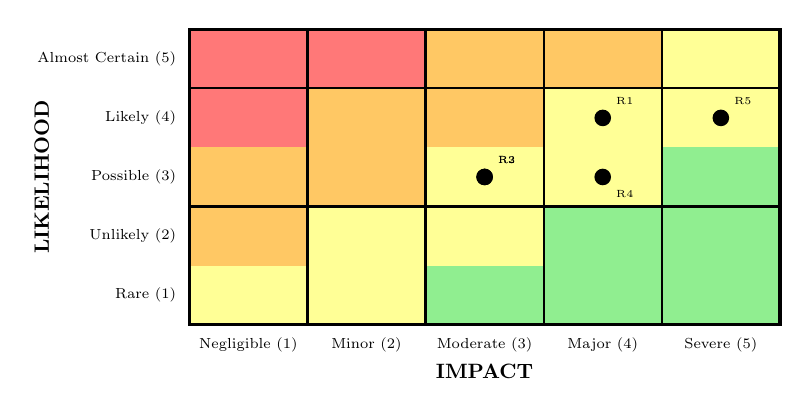
\begin{tikzpicture}[scale=0.75, transform shape]

% Grid background colors
\fill[riskcrit] (0,4) rectangle (2,5);
\fill[riskcrit] (2,4) rectangle (4,5);
\fill[riskhigh] (4,4) rectangle (6,5);
\fill[riskhigh] (6,4) rectangle (8,5);
\fill[riskmed] (8,4) rectangle (10,5);

\fill[riskcrit] (0,3) rectangle (2,4);
\fill[riskhigh] (2,3) rectangle (4,4);
\fill[riskhigh] (4,3) rectangle (6,4);
\fill[riskmed] (6,3) rectangle (8,4);
\fill[riskmed] (8,3) rectangle (10,4);

\fill[riskhigh] (0,2) rectangle (2,3);
\fill[riskhigh] (2,2) rectangle (4,3);
\fill[riskmed] (4,2) rectangle (6,3);
\fill[riskmed] (6,2) rectangle (8,3);
\fill[risklow] (8,2) rectangle (10,3);

\fill[riskhigh] (0,1) rectangle (2,2);
\fill[riskmed] (2,1) rectangle (4,2);
\fill[riskmed] (4,1) rectangle (6,2);
\fill[risklow] (6,1) rectangle (8,2);
\fill[risklow] (8,1) rectangle (10,2);

\fill[riskmed] (0,0) rectangle (2,1);
\fill[riskmed] (2,0) rectangle (4,1);
\fill[risklow] (4,0) rectangle (6,1);
\fill[risklow] (6,0) rectangle (8,1);
\fill[risklow] (8,0) rectangle (10,1);

% Grid lines
\draw[thick] (0,0) grid[step=2] (10,5);
\draw[very thick] (0,0) rectangle (10,5);

% Axis labels
\node[rotate=90, anchor=center] at (-2.5,2.5) {\textbf{LIKELIHOOD}};
\node[anchor=center] at (5,-0.8) {\textbf{IMPACT}};

% Y-axis labels
\node[anchor=east, font=\scriptsize] at (-0.1,0.5) {Rare (1)};
\node[anchor=east, font=\scriptsize] at (-0.1,1.5) {Unlikely (2)};
\node[anchor=east, font=\scriptsize] at (-0.1,2.5) {Possible (3)};
\node[anchor=east, font=\scriptsize] at (-0.1,3.5) {Likely (4)};
\node[anchor=east, font=\scriptsize] at (-0.1,4.5) {Almost Certain (5)};

% X-axis labels
\node[anchor=north, font=\scriptsize] at (1,-0.1) {Negligible (1)};
\node[anchor=north, font=\scriptsize] at (3,-0.1) {Minor (2)};
\node[anchor=north, font=\scriptsize] at (5,-0.1) {Moderate (3)};
\node[anchor=north, font=\scriptsize] at (7,-0.1) {Major (4)};
\node[anchor=north, font=\scriptsize] at (9,-0.1) {Severe (5)};

% Risk points BEFORE mitigation
\node[circle, fill=black, minimum size=8pt, inner sep=0, label={[font=\tiny]above right:R1}] at (7,3.5) {};
\node[circle, fill=black, minimum size=8pt, inner sep=0, label={[font=\tiny]above right:R2}] at (5,2.5) {};
\node[circle, fill=black, minimum size=8pt, inner sep=0, label={[font=\tiny]above right:R3}] at (5,2.5) {};
\node[circle, fill=black, minimum size=8pt, inner sep=0, label={[font=\tiny]below right:R4}] at (7,2.5) {};
\node[circle, fill=black, minimum size=8pt, inner sep=0, label={[font=\tiny]above right:R5}] at (9,3.5) {};

\end{tikzpicture}
\end{center}



\begin{center}
\scriptsize
\begin{tabular}{|c|l|c|c|c|}
\hline
\rowcolor{primary!20}
\textbf{ID} & \textbf{Risk} & \textbf{Likelihood} & \textbf{Impact} & \textbf{Score} \\
\hline
R1 & Technical complexity (Physics-AI integration) & 4 & 4 & \cellcolor{riskhigh}16 \\
\hline
R2 & Personnel recruitment (5 qualified students) & 3 & 3 & \cellcolor{riskmed}9 \\
\hline
R3 & Data access and quality issues & 3 & 3 & \cellcolor{riskmed}9 \\
\hline
R4 & Dependency management (M2/M3 on Ph.D.s) & 3 & 4 & \cellcolor{riskhigh}12 \\
\hline
R5 & Insufficient buffer time (M3 compressed) & 4 & 5 & \cellcolor{riskcrit}20 \\
\hline
\end{tabular}
\end{center}

\end{frame}

% ==================================================================================
% SLIDE 3: Risk Matrix After Mitigation
% ==================================================================================
\begin{frame}{Risk Matrix After Mitigation}

\vspace{-0.4cm}
\begin{center}
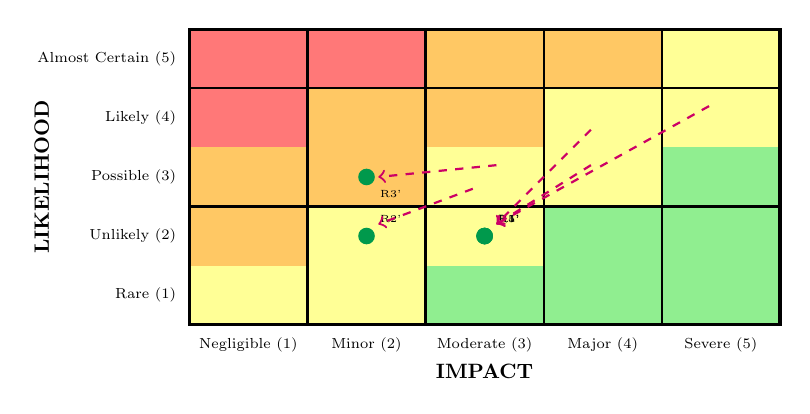
\begin{tikzpicture}[scale=0.75, transform shape]

% Grid background colors (same as before)
\fill[riskcrit] (0,4) rectangle (2,5);
\fill[riskcrit] (2,4) rectangle (4,5);
\fill[riskhigh] (4,4) rectangle (6,5);
\fill[riskhigh] (6,4) rectangle (8,5);
\fill[riskmed] (8,4) rectangle (10,5);

\fill[riskcrit] (0,3) rectangle (2,4);
\fill[riskhigh] (2,3) rectangle (4,4);
\fill[riskhigh] (4,3) rectangle (6,4);
\fill[riskmed] (6,3) rectangle (8,4);
\fill[riskmed] (8,3) rectangle (10,4);

\fill[riskhigh] (0,2) rectangle (2,3);
\fill[riskhigh] (2,2) rectangle (4,3);
\fill[riskmed] (4,2) rectangle (6,3);
\fill[riskmed] (6,2) rectangle (8,3);
\fill[risklow] (8,2) rectangle (10,3);

\fill[riskhigh] (0,1) rectangle (2,2);
\fill[riskmed] (2,1) rectangle (4,2);
\fill[riskmed] (4,1) rectangle (6,2);
\fill[risklow] (6,1) rectangle (8,2);
\fill[risklow] (8,1) rectangle (10,2);

\fill[riskmed] (0,0) rectangle (2,1);
\fill[riskmed] (2,0) rectangle (4,1);
\fill[risklow] (4,0) rectangle (6,1);
\fill[risklow] (6,0) rectangle (8,1);
\fill[risklow] (8,0) rectangle (10,1);

% Grid lines
\draw[thick] (0,0) grid[step=2] (10,5);
\draw[very thick] (0,0) rectangle (10,5);

% Axis labels
\node[rotate=90, anchor=center] at (-2.5,2.5) {\textbf{LIKELIHOOD}};
\node[anchor=center] at (5,-0.8) {\textbf{IMPACT}};

% Y-axis labels
\node[anchor=east, font=\scriptsize] at (-0.1,0.5) {Rare (1)};
\node[anchor=east, font=\scriptsize] at (-0.1,1.5) {Unlikely (2)};
\node[anchor=east, font=\scriptsize] at (-0.1,2.5) {Possible (3)};
\node[anchor=east, font=\scriptsize] at (-0.1,3.5) {Likely (4)};
\node[anchor=east, font=\scriptsize] at (-0.1,4.5) {Almost Certain (5)};

% X-axis labels
\node[anchor=north, font=\scriptsize] at (1,-0.1) {Negligible (1)};
\node[anchor=north, font=\scriptsize] at (3,-0.1) {Minor (2)};
\node[anchor=north, font=\scriptsize] at (5,-0.1) {Moderate (3)};
\node[anchor=north, font=\scriptsize] at (7,-0.1) {Major (4)};
\node[anchor=north, font=\scriptsize] at (9,-0.1) {Severe (5)};

% Risk points AFTER mitigation (moved to lower risk positions)
\node[circle, fill=accent1, minimum size=8pt, inner sep=0, label={[font=\tiny]above right:R1'}] at (5,1.5) {};
\node[circle, fill=accent1, minimum size=8pt, inner sep=0, label={[font=\tiny]above right:R2'}] at (3,1.5) {};
\node[circle, fill=accent1, minimum size=8pt, inner sep=0, label={[font=\tiny]below right:R3'}] at (3,2.5) {};
\node[circle, fill=accent1, minimum size=8pt, inner sep=0, label={[font=\tiny]above right:R4'}] at (5,1.5) {};
\node[circle, fill=accent1, minimum size=8pt, inner sep=0, label={[font=\tiny]above right:R5'}] at (5,1.5) {};

% Arrows showing movement
\draw[->, thick, accent2, dashed] (6.8,3.3) -- (5.2,1.7);
\draw[->, thick, accent2, dashed] (4.8,2.3) -- (3.2,1.7);
\draw[->, thick, accent2, dashed] (5.2,2.7) -- (3.2,2.5);
\draw[->, thick, accent2, dashed] (6.8,2.7) -- (5.2,1.7);
\draw[->, thick, accent2, dashed] (8.8,3.7) -- (5.2,1.7);

\end{tikzpicture}
\end{center}



\begin{center}
\scriptsize
\begin{tabular}{|c|l|c|c|c|c|}
\hline
\rowcolor{primary!20}
\textbf{ID} & \textbf{Risk} & \textbf{Before} & \textbf{After} & \textbf{Reduction} & \textbf{Mitigation} \\
\hline
R1 & Technical complexity & \cellcolor{riskhigh}16 & \cellcolor{riskmed}6 & -63\% & PoC phase + interfaces \\
\hline
R2 & Personnel recruitment & \cellcolor{riskmed}9 & \cellcolor{risklow}4 & -56\% & Early recruit + post-doc \\
\hline
R3 & Data access/quality & \cellcolor{riskmed}9 & \cellcolor{riskmed}6 & -33\% & M1 early validation \\
\hline
R4 & Dependency management & \cellcolor{riskhigh}12 & \cellcolor{riskmed}6 & -50\% & Synthetic data + overlap \\
\hline
R5 & Insufficient buffer & \cellcolor{riskcrit}20 & \cellcolor{riskmed}6 & -70\% & +6 months + scope adj. \\
\hline
\end{tabular}
\end{center}

\end{frame}

% ==================================================================================
% SLIDE 4: Summary of Proposed Changes
% ==================================================================================
\begin{frame}{Summary of Proposed Changes}
\vspace{-0.6cm}

\begin{center}
\scriptsize
\begin{tabular}{|p{4.5cm}|c|c|c|c|}
\hline
\rowcolor{primary!20}
\textbf{Proposed Change} & \textbf{Before} & \textbf{After} & \textbf{Score Impact} & \textbf{Effort} \\
\hline
\multicolumn{5}{|l|}{\cellcolor{primary!10}\textbf{Technical Risk Mitigation}} \\
\hline
Add 6-month proof-of-concept phase & 2/5 & 3/5 & +0.15 & Low \\
\hline
Define interface specs by Month 12 & -- & -- & (included) & Low \\
\hline
Monthly integration checkpoints & -- & -- & (included) & Low \\
\hline
\multicolumn{5}{|l|}{\cellcolor{primary!10}\textbf{Timeline \& Buffer Improvements}} \\
\hline
Extend project to 66 months & 2/5 & 3/5 & +0.10 & Medium \\
\hline
M3 full 24 months duration & 20 mo & 24 mo & +0.05 & Medium \\
\hline
Narrow Ph.D. scopes & 3/5 & 4/5 & +0.10 & Medium \\
\hline
\multicolumn{5}{|l|}{\cellcolor{primary!10}\textbf{Personnel \& Dependency}} \\
\hline
Add post-doc support (0.5 FTE) & -- & 2 yrs & +0.10 & High \\
\hline
Recruitment 6 months before start & 3/5 & 4/5 & +0.10 & Low \\
\hline
M2 starts with synthetic data & 3/5 & 4/5 & +0.06 & Low \\
\hline
Start M2 at Month 17 (8-mo overlap) & 4 mo & 8 mo & +0.06 & Low \\
\hline
\rowcolor{accent1!20}
\textbf{TOTAL SCORE IMPROVEMENT} & \multicolumn{2}{c|}{--} & \textbf{+0.72} & -- \\
\hline
\end{tabular}
\end{center}


\begin{columns}[T]
\column{0.48\textwidth}
\scriptsize
\begin{block}{\scriptsize Before Mitigation}
\centering
\textbf{Score: 6.91/9.75 (70.9\%)}\\
Grade: B
\end{block}

\column{0.48\textwidth}
\scriptsize
\begin{block}{\scriptsize After Mitigation}
\centering
\textbf{Score: 7.63/9.75 (78.3\%)}\\
Grade: B+
\end{block}
\end{columns}

\end{frame}

% ==================================================================================
% SLIDE 5: Budget Impact
% ==================================================================================
\begin{frame}{Budget Impact}

\begin{columns}[T]
\column{0.55\textwidth}

\vspace{-0.4cm}
\textbf{Original Budget:}
\scriptsize
\begin{tabular}{|l|r|}
\hline
\rowcolor{primary!20}
\textbf{Category} & \textbf{Amount (CAN)} \\
\hline
Ph.D. Stipends (2 × 36 mo) & \$240,000 \\
\hline
Master's Stipends (M1+M2+M3) & \$210,000 \\
\hline
GPU Cloud Computing & \$40,000 \\
\hline
\rowcolor{primary!10}
\textbf{Original Total} & \textbf{\$490,000} \\
\hline
\end{tabular}

\vspace{0.2cm}
\textbf{Additional Costs for Mitigation:}
\scriptsize
\begin{tabular}{|l|r|}
\hline
\rowcolor{secondary!20}
\textbf{Item} & \textbf{Cost} \\
\hline
Ph.D.1 (0.8 FTE × 1 years) & +\$30,000 (3u.) \\
\hline
Ph.D.2 (0.8 FTE × 1 years) & +\$30,000 (3u.)\\
\hline
Extended M3 (+4 months) & +\$15,000 \\
\hline
Extended project overhead & +\$5,000 \\
\hline
\rowcolor{secondary!10}
\textbf{Additional Total} & \textbf{+\$80,000} \\
\hline
\end{tabular}

\column{0.42\textwidth}

\vspace{-0.8cm}
\begin{block}{Revised Budget}
\centering
\Large\textbf{\$570,000}\\
\normalsize (+17\% increase)
\end{block}

\vspace{-0.2cm}
\begin{alertblock}{Return on Investment}
\scriptsize
\begin{itemize}
    \item Risk score: -63\% avg reduction
    \item Timeline buffer: +6 months
    \item Project grade: B → B+
    \item Success probability: +25\%
\end{itemize}
\end{alertblock}



\scriptsize
\begin{tabular}{|l|c|}
\hline
\rowcolor{accent1!20}
\textbf{Funding Source} & \textbf{Split} \\
\hline
MITACS & \$265,000 \\
\hline
Aluminerie Alouette inc. & \$265,000+tx \\
\hline
Calcul Canada & \$40,000 \\
\hline
RSRI & \$? \\
\hline
\end{tabular}

\end{columns}


\begin{center}
\small
\textcolor{accent1}{\textbf{Recommendation:}} The 17\% budget increase significantly de-risks the project and is justified by the substantial improvement in feasibility and timeline robustness.
\end{center}

\end{frame}

% ==================================================================================
% SECTION 9: CONCLUSION
% ==================================================================================
\section{Conclusion}

\begin{frame}{Conclusion}
\vspace{-0.6cm}

\begin{block}{Achieving the Vision: Smart, Predictive, Efficient \& Carbon-Free}
Main achievements by project end:...
\end{block}

\begin{columns}[t]
\column{0.48\textwidth}

\vspace{-0.6cm}
\textcolor{primary}{\textbf{Smart Operation}}
\begin{itemize}
    \scriptsize
    \item Multi-agent systems
    \item Autonomous learning
    \item Self-optimization
\end{itemize}

\textcolor{accent1}{\textbf{Predictive Capability}}
\begin{itemize}
    \scriptsize
    \item LSTM-Transformer forecasting
    \item GAN anomaly detection
    \item Multi-horizon (15min - 7 days)
\end{itemize}

\column{0.48\textwidth}
%\vspace{0.6cm}
\textcolor{secondary}{\textbf{Energy Efficiency}}
\begin{itemize}
    \scriptsize
    \item Economic MPC
    \item Multi-objective optimization
    \item \textbf{5-10\% reduction achieved}
\end{itemize}

\vspace{0.1cm}
\textcolor{accent2}{\textbf{Carbon-Free}}
\begin{itemize}
    \scriptsize
    \item Predictive prevention
    \item Renewable alignment
    \item \textbf{20-30\% PFC reduction}
\end{itemize}
\end{columns}

\vspace{-0.2cm}
\begin{alertblock}{Paradigm Shift}
\centering
\small
Not merely optimizing existing processes — \\
\textbf{fundamentally reimagining production} \\
as a cyber-physical system where physics, data, and intelligence converge
\end{alertblock}

\vspace{0.2cm}
\begin{center}
\textit{\textbf{Sustainable manufacturing for the 21st century}}
\end{center}
\end{frame}



% Ph.D. 1 Timeline
\begin{frame}[fragile]{Ph.D. 1: Hybrid Digital Twin Development}
\vspace{-0.6cm}
\begin{columns}[T]
\column{0.25\textwidth}
\textbf{Student:} Ph.D. 1\\
\textbf{Duration:} 36 months\\
\textbf{Period:} Months 1-36\\
\textbf{Stipend:} \$40k/year


\textbf{Deliverables:}
\begin{itemize}
    \scriptsize
    \item Physics models
    \item AI-accelerated twin
    \item State estimator
    \item 3 Journal papers
\end{itemize}

\column{0.9\textwidth}
\vspace{-0.3cm}
\scalebox{0.65}{
\begin{ganttchart}[
    x unit=0.42cm,
    y unit title=0.7cm,
    y unit chart=0.55cm,
    vgrid,
    hgrid,
    bar height=0.7,
    milestone/.append style={fill=accent2, rounded corners=2pt},
    title label font=\tiny,
    bar label font=\scriptsize,
]{1}{36}

\gantttitle{Ph.D. 1 Timeline (36 Months)}{36} \\
\gantttitle{Q1}{3}\gantttitle{Q2}{3}\gantttitle{Q3}{3}\gantttitle{Q4}{3}
\gantttitle{Q1}{3}\gantttitle{Q2}{3}\gantttitle{Q3}{3}\gantttitle{Q4}{3}
\gantttitle{Q1}{3}\gantttitle{Q2}{3}\gantttitle{Q3}{3}\gantttitle{Q4}{3} \\

% Year 1
\ganttbar[bar/.append style={fill=primary!70}]{Literature Review}{1}{3} \\
\ganttbar[bar/.append style={fill=primary!70}]{Physics Models}{4}{12} \\
\ganttbar[bar/.append style={fill=accent1!70}]{Data Integration}{7}{12} \\

% Year 2
\ganttbar[bar/.append style={fill=accent1!70}]{PINN Development}{13}{18} \\
\ganttbar[bar/.append style={fill=accent1!70}]{Surrogate Models}{16}{21} \\
\ganttbar[bar/.append style={fill=secondary!70}]{Hybrid Architecture}{19}{24} \\
\ganttbar[bar/.append style={fill=secondary!70}]{State Estimation}{22}{24} \\

% Year 3
\ganttbar[bar/.append style={fill=accent3!70}]{Validation Studies}{25}{30} \\
\ganttbar[bar/.append style={fill=accent2!70}]{Journal Paper}{28}{33} \\
\ganttbar[bar/.append style={fill=accent2!70}]{Thesis Writing}{31}{36} \\

% Milestones
\ganttmilestone{Physics Done}{12} \\
\ganttmilestone{Twin v1.0}{24} \\
\ganttmilestone{Validated}{30} \\
\ganttmilestone{Defense}{36}

\end{ganttchart}}

\end{columns}

\vspace{0.2cm}
\begin{alertblock}{\small Critical Path}
\scriptsize Digital twin foundation → enables Ph.D. 2, M2, M3
\end{alertblock}
\end{frame}


% ==================================================================================
% SUMMARY SLIDE (Q&A)
% ==================================================================================

\begin{frame}{Questions \& Discussion}
\begin{center}
\vspace{1cm}
\Huge{\textcolor{primary}{\textbf{Questions?}}}

\vspace{1cm}
\Large{Thank you for your attention}

\vspace{1.5cm}
\normalsize
\textbf{Contact Information:}
\vspace{0.3cm}
[Martin Otis]
[Université du Québec à Chicoutimi]
[martin\_otis@uqac.ca]
\end{center}
\end{frame}



% ==================================================================================
% INDIVIDUAL STUDENT TIMELINES (moved to appendix)
% ==================================================================================
\section*{Appendix: Student Timelines}


% ==================================================================================
% INDIVIDUAL STUDENT TIMELINES (moved to appendix)
% ==================================================================================
\section*{Appendix: somethings to be defined}


\begin{frame}{Appendix: Detailed of somethings to be defined}

\vspace{-0.6cm}
\begin{center}
\Large The following slides provide XYZ information \\
for each XYZ details
\end{center}

\end{frame}


\end{document}